\documentclass{beamer}

% Top-aligning columns within a top-aligned frame
% https://tex.stackexchange.com/questions/16447/beamer-top-aligning-columns-within-a-top-aligned-frame
\makeatletter
\newenvironment{myitemize}{%
   \setlength{\topsep}{0pt}
   \setlength{\partopsep}{0pt}
   \renewcommand*{\@listi}{\leftmargin\leftmargini \parsep\z@ \topsep\z@ \itemsep\z@}
   \let\@listI\@listi
   \itemize
}{\enditemize}
\makeatother  

\usepackage[USenglish]{babel}
\usepackage[utf8]{inputenc}
\usepackage{amssymb, amsmath}
\usepackage{bm}
\usepackage{color}
\usepackage{tikz}
\usepackage{url}

\definecolor{links}{HTML}{2A1B81}
\hypersetup{colorlinks,linkcolor=,urlcolor=links}

\usetheme{Boadilla}

\bibliographystyle{apalike}
% make bibliography entries smaller
%\renewcommand\bibfont{\scriptsize}
% Now get rid of all the colours
\setbeamercolor*{bibliography entry title}{fg=black}
\setbeamercolor*{bibliography entry author}{fg=black}
\setbeamercolor*{bibliography entry location}{fg=black}
\setbeamercolor*{bibliography entry note}{fg=black}

\newcommand{\lnorm}[1]{\left\lVert#1\right\rVert^2}
\newcommand{\norm}[1]{\left\lVert#1\right\rVert}

% and kill the abominable icon
\setbeamertemplate{bibliography item}{}

\begin{document}
\title[BigBird]{Big Bird: Transformers for Longer Sequences}  
\author{Radek Bartyzal}
\date{1. 9. 2020} 
\institute{GLAMI AI}

\frame{\titlepage} 

%--------- END Frame 12 -------------
\begin{frame}{Motivation}

\textbf{What is old:}
\begin{itemize}
\item Transformers are good
\item self-attention is crucial for transformers
\item self-attention = $O(n^2)$ memory + comp. requirements
\item typical max sentence length = 512 tokens
\end{itemize}

\vfill

\textbf{What is new:}
\begin{itemize}
\item is the $O(n^2)$ necessary?
\item BigBird claims to replace self-attention with BigBird attention that is $O(n)$
\end{itemize}

\end{frame}
%--------- END Frame 12 -------------
\begin{frame}{Previous works}
A lot of papers reducing the complexity of self-attention, notably:
\begin{itemize}
\item Synthesizer: synthesize the result of the full-attention
\item Linformer: approximate full-attention by 2 low-rank matrices
\item Longformer: Window + Global attention, 2 months earlier
\item $\implies$ BigBird = Longformer + Random attention
\end{itemize}
\end{frame}
%--------- END Frame 12 -------------
\begin{frame}{BigBird Attention}

\begin{figure}[h]
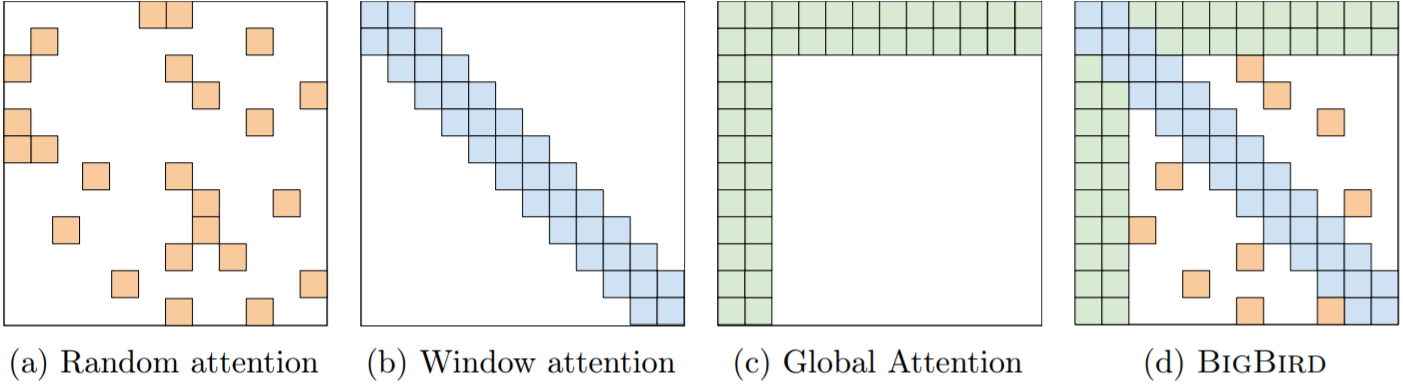
\includegraphics[width=\textwidth]{img/attention}
\caption{Building blocks of the attention mechanism used in BigBird. White color indicates absence of attention. (a) random attention with $r$ = 2, (b) sliding window attention with $w$ = 3 (c) global attention with $g$ = 2. (d) the combined BigBird model.}
\end{figure}

\begin{itemize}
\item \textbf{Random}: each token attends to $r$ random other tokens
\item \textbf{Window}: all tokens attend to their surrounding tokens = similar to Convolution
\item \textbf{Global}: certain tokens (e.g. CLS) receive from all and send to all

\end{itemize}

\end{frame}
%--------- END Frame 12 -------------
\begin{frame}{BigBird attention}

\begin{itemize}
\item $r$, $w$, $g$ is fixed = constant = hyperparameter
\item therefore it is $O(n)$
\item capable of simulating full self-attention
\item the random mask is different for each sentence but fixed through the layers
\end{itemize}
\end{frame}

%--------- END Frame 12 -------------
\begin{frame}{Attention as graph}

\begin{itemize}
\item Random attention = graph where each edge is independently chosen with a fixed probability.

\item In such a random graph with just $\Theta(n)$ edges, the shortest path between any two nodes is logarithmic in the number of nodes.

\item $\implies$ quick mixing of information between nodes in following layers

\item however in worst case it takes $n$ layers to simulate 1 full self-attention layer

\item $\implies$ in worst case we would have to have $n$ $\times$ more layers = $O(n^2)$ again

\item $\implies$ not truly $O(n)$ attention replacement
\end{itemize}


\end{frame}
%--------- END Frame 12 -------------
\begin{frame}{Global attention is necessary}
\begin{figure}[h]
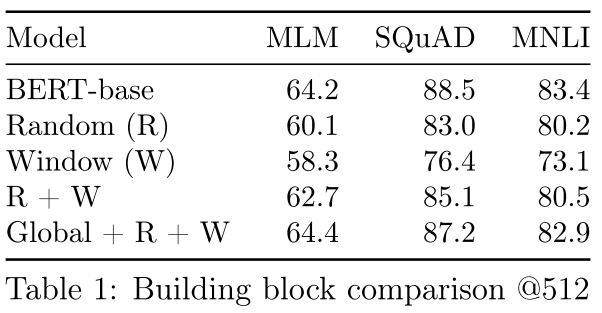
\includegraphics[width=0.7\textwidth]{img/blocks}
\caption{Random blocks and local window were insufficient in capturing all the context necessary to compete with the performance of BERT.}
\end{figure}
\end{frame}
%--------- END Frame 12 -------------
\begin{frame}{Cache optimization}
\begin{figure}[h]
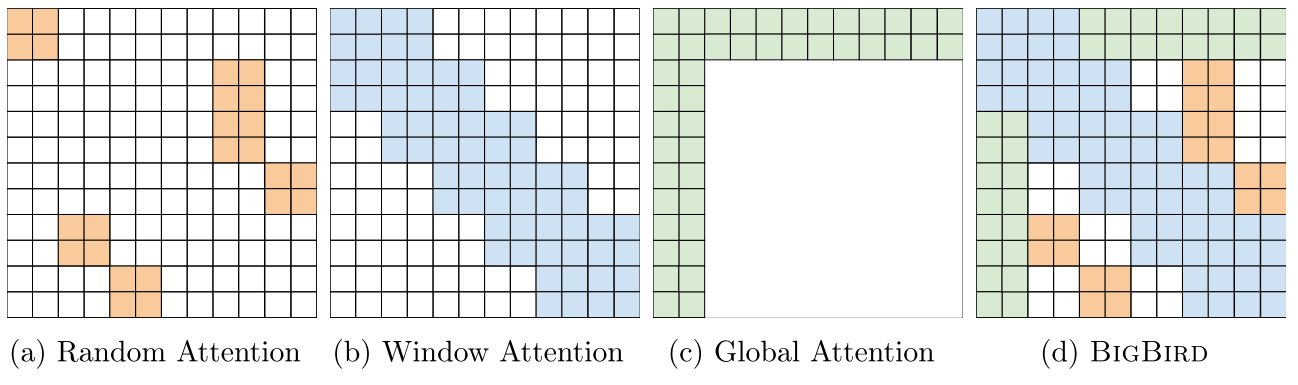
\includegraphics[width=\textwidth]{img/cache}
\caption{Building blocks of the block-attention mechanism used in BigBird with block size = 2. This implies the attention matrix is split into blocks of size $2 \times 2$. All the previous BigBird parameters work on each block as a unit.}
\end{figure}
\end{frame}
%--------- END Frame 12 -------------
\begin{frame}{Question Answering results}
\begin{figure}[h]
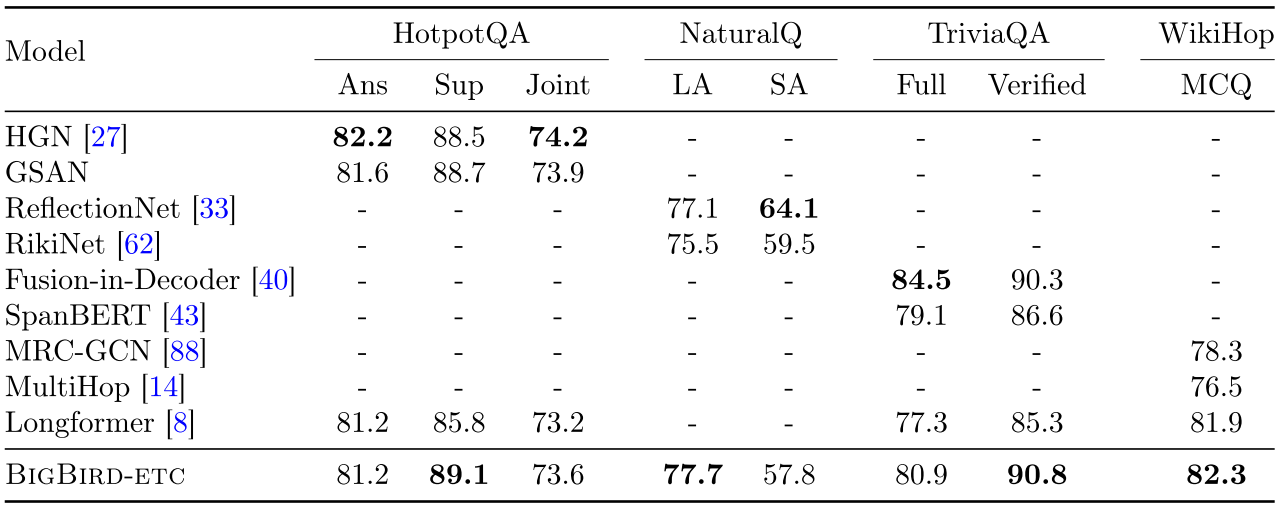
\includegraphics[width=\textwidth]{img/qa_res}
\caption{Fine-tuning results on Test set for QA tasks. For Natural Questions Long Answer (LA), TriviaQA Verified, and WikiHop, \textbf{BigBird-ETC is the new state-of-the-art}.}
\end{figure}
\end{frame}
%--------- END Frame 12 -------------
\begin{frame}{Question Answering params = no random attention?}
\begin{figure}[h]
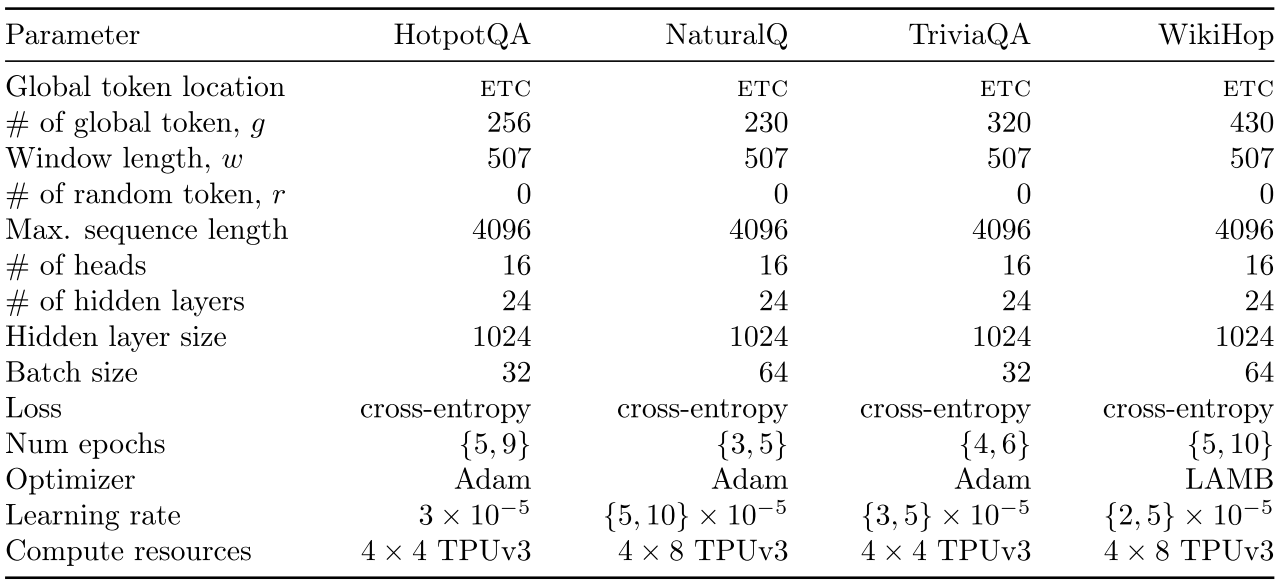
\includegraphics[width=\textwidth]{img/qa_params}
\caption{Hyperparameters of large BigBird model for Question Answering submitted for test.}
\end{figure}
\end{frame}
%--------- END Frame 12 -------------
\begin{frame}{Conclusion}
\begin{itemize}
\item a lot of engineering to optimize Window + Global + Random attention
\item allows longer sequence length and larger batch size
\item $\implies$ which brings improvements on almost all tasks
\end{itemize}
\end{frame}

%--------- END Frame 12 -------------
\begin{frame}{Sources}
\begin{thebibliography}{0}

  \bibitem[1]{cit:paper} 1. Zaheer, Manzil, et al. "Big bird: Transformers for longer sequences." arXiv preprint arXiv:2007.14062 (2020). \url{https://arxiv.org/abs/2007.14062v1} 

  
\end{thebibliography}
\end{frame} 
\end{document}
